\documentclass[12pt]{article}
\usepackage[utf8]{inputenc}
\usepackage{array}
\usepackage{xcolor}
\usepackage{graphicx}
\usepackage{mathtools}
\usepackage{amsmath}
\usepackage{multicol}
\usepackage{eqnarray}
\usepackage{wrapfig}


\usepackage{natbib}
\usepackage{hyperref}
\hypersetup{
	colorlinks=true,
	linkcolor=black,
	filecolor=mangeta,      
	urlcolor=blue,
	pdftitle={Overleaf Example},
	pdfpagemode=FullScreen,
}

\usepackage[margin=0.6in]{geometry}

\title{52nd—24th INTERNATIONAL-RUDOLF ORTVAY \\ PROBLEM SOLVING CONTEST IN PHYSICS \\ Problem 2}
\author{Nguyen Thanh Long}
\date{\today}

\begin{document}
	
\maketitle
	
\noindent We can see that the Lagrangian will be:
$$ L = r^2 \sin^2 \theta \dot{\varphi}^2 + r^2 \dot{\theta}^2 + \dot{r}^2 .$$
If we let $x=r$, $y = \sin \theta $ (If $y^2>1$, $\theta$ may be a complex number) and $z = \varphi $. If we multiphy this Lagrangian by a constant $\frac{m}{2}$, this exactly is the Lagrangian of a free particle, with mass $m$, moving non-relativistic in the spherical coordinate system. Therefore, in the same way, we can build a coordinate system $(x_1, x_2, x_3)$ in order to the Lagrangian be quadratic form with: 
\begin{align*}
	x_1 & = x \sqrt{1-y^2} \cos ( z) \\
	x_2 & = x \sqrt{1-y^2} \sin ( z) \\
	x_3 & = xy.
\end{align*}	

\noindent The new Lagrangian will be:

$$ L = \dot{x}_1^2 + \dot{x}_2^2 + \dot{x}_3^2 .$$
The Euler-Lagrange equation with $x_1$:

$$ \frac{d}{dt} \left( \frac{ \partial L}{\partial \dot{x}_1 } \right) = \frac{ \partial L}{ \partial x_1} \Rightarrow 2 \frac{d \dot{x}_1}{dt} = 0 \Rightarrow \dot{x}_1 = C_{1a} \Rightarrow x_1 = C_{1a} t + C_{1b}.$$
Where $C_{1a}$ and $C_{1b}$ is a constant. Similar, we have $x_2 = C_{2a} t + C_{2b}$ and $ x_3 = C_{3a} t + C_{3b}$.

\noindent Now, we write again $x$, $y$, $z$ and receive the general solution of Lagrangian:

\begin{align*}
	x & = \sqrt{x_1^2 + x_2^2 + x_3^2} = \sqrt{\left( C_{1a} t + C_{1b} \right)^2 + \left( C_{2a} t + C_{2b} \right)^2 +\left( C_{3a} t + C_{3b} \right)^2 }. \\
	y & = \frac{x_3}{\sqrt{x_1^2 + x_2^2 + x_3^2}} = \frac{C_{3a} t + C_{3b}}{\sqrt{\left( C_{1a} t + C_{1b} \right)^2 + \left( C_{2a} t + C_{2b} \right)^2 +\left( C_{3a} t + C_{3b} \right)^2 }} . \\
	z & = \arctan \left( \frac{x_2}{x_1} \right) = \arctan \left( \frac{ C_{2a} t + C_{2b} }{ C_{1a} t + C_{1b} } \right) .
\end{align*}

\noindent With the values of $x$, $\dot{x}$, $y$, $\dot{y}$, $z$, $\dot{z}$ at any time, we have 6 equations to find 6 constant: $C_{1a}$, $C_{1b}$, $C_{2a}$, $C_{2b}$, $C_{3a}$, $C_{3b}$.

\newpage

\noindent Using the result we have found, if we choose $(x_1, x_2, x_3)$ is a Canonical basis (or Descartes coordinate for three dimensions), $(x, y, z)$ will be a new coordinate system as shown below (in Figure \ref{Fig P2}).

\begin{figure}[!htb]
	\centering
	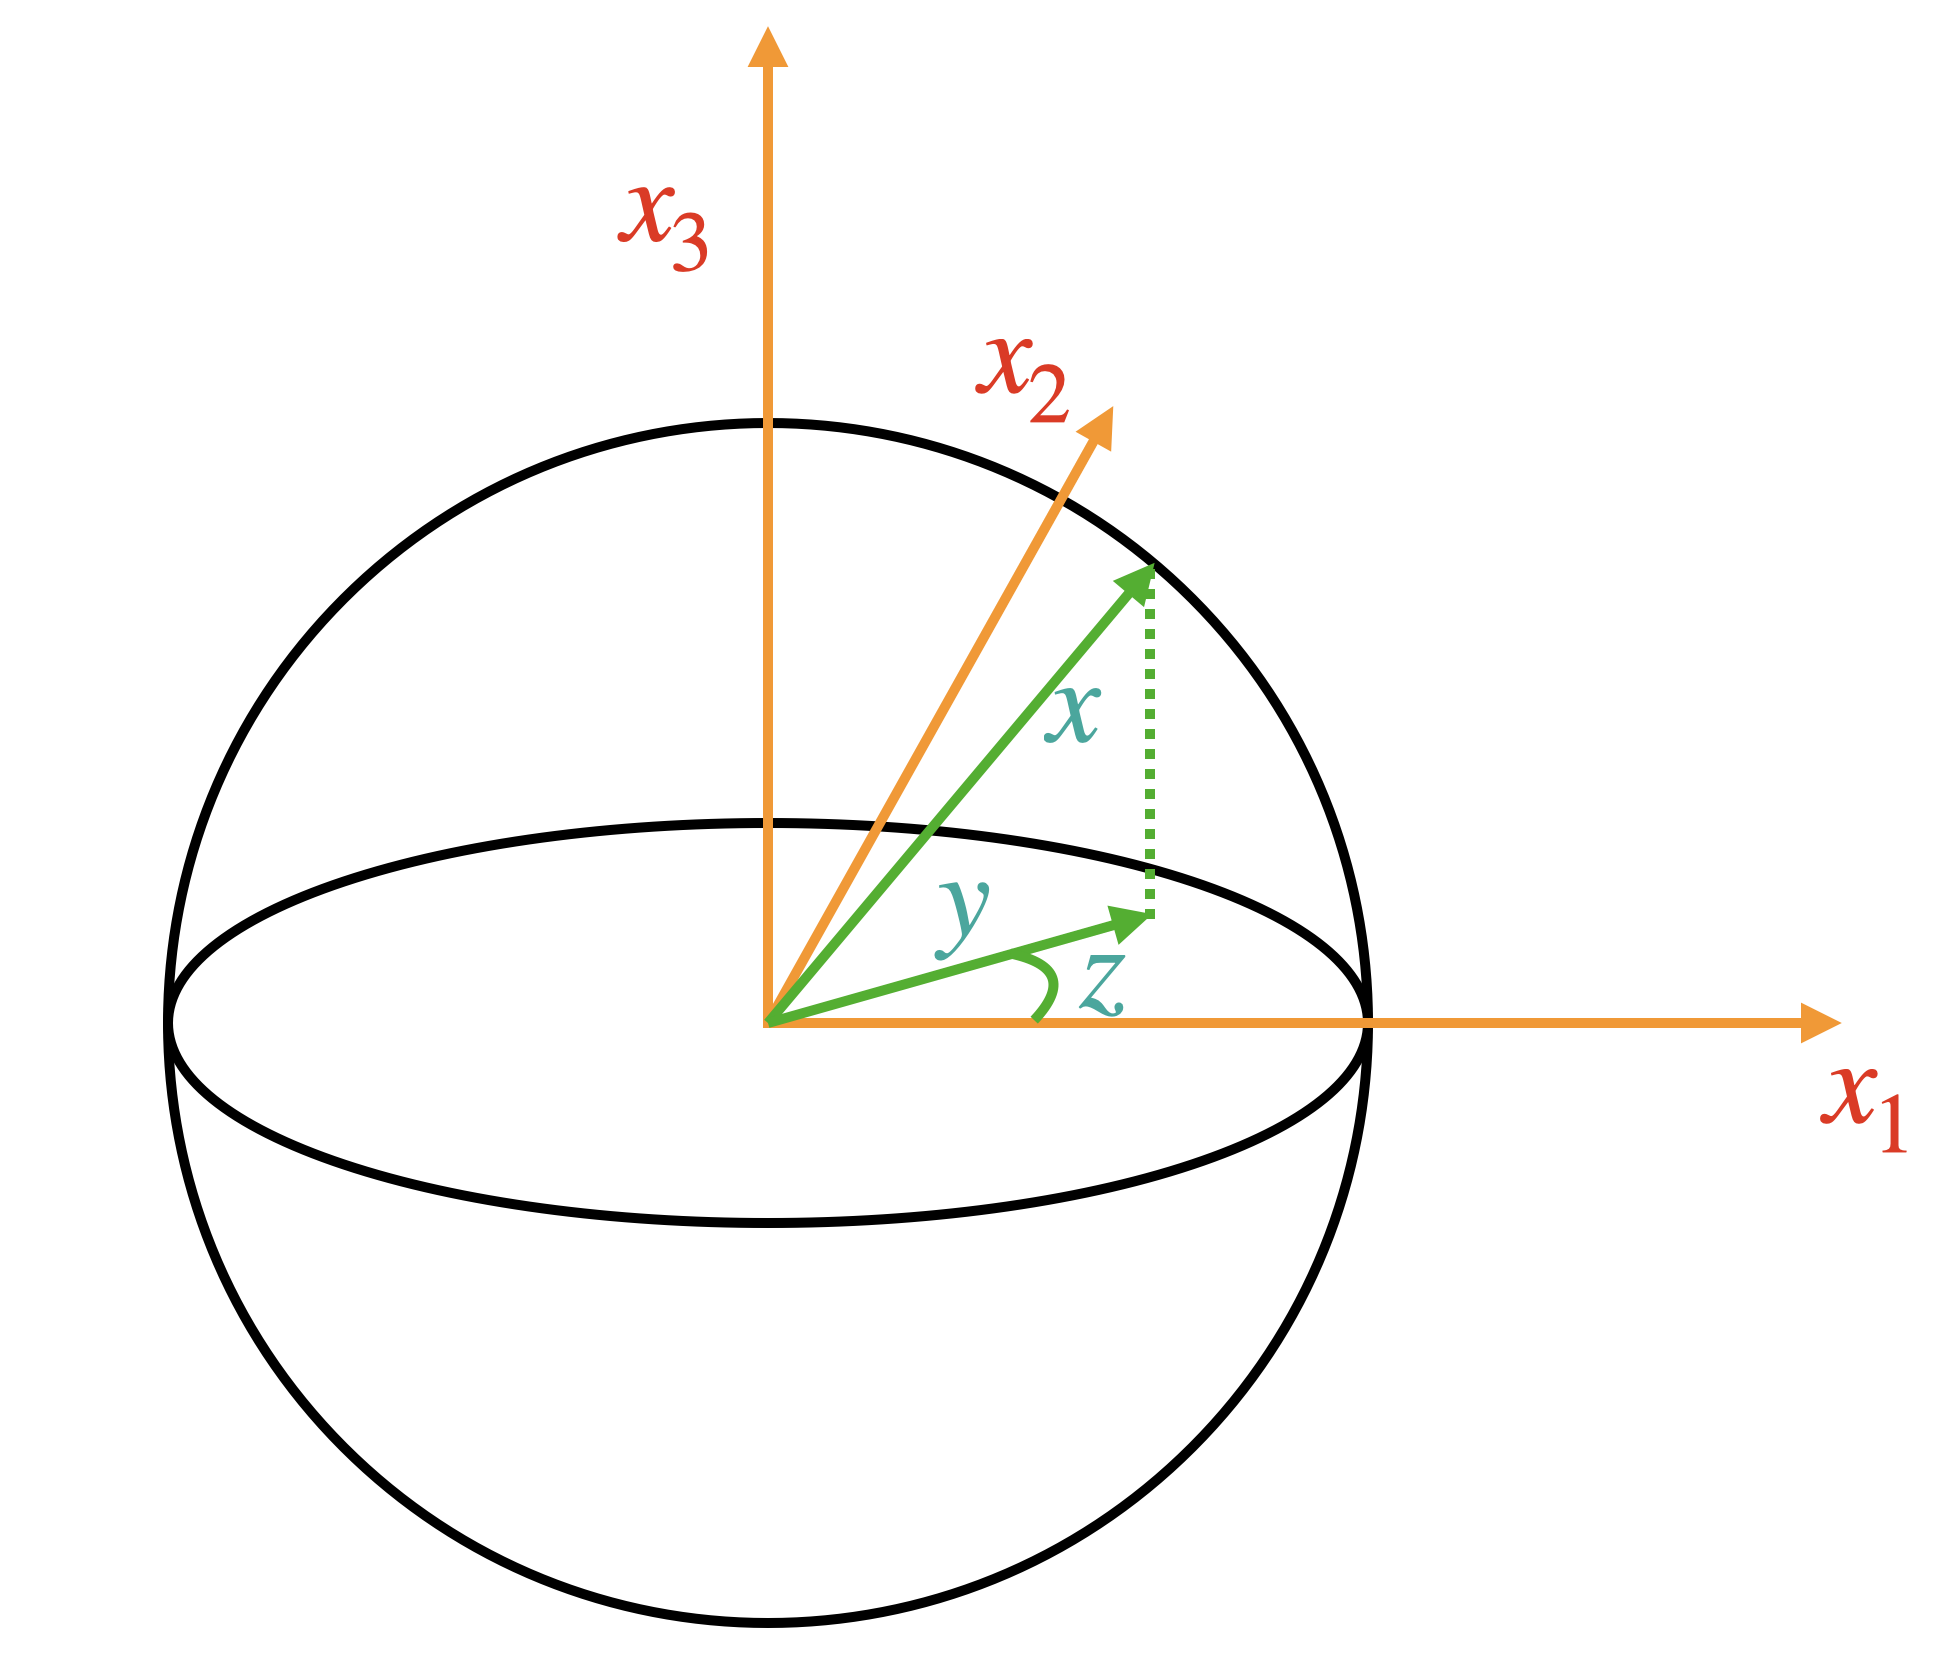
\includegraphics[width=0.7\textwidth]{Fig P2.png}
	\caption{The coordinate system of this problems}
	\label{Fig P2}
\end{figure}	

\noindent Remember, in this problem, the Lagragian does not have any explicit dependence on $z$, so we only can find $\dot{z}$ and when we performance $z$, may be we need a constant $\phi$ so as to: $x_1 = x \sqrt{ 1 - y^2 } \cos (z - \phi)$, $x_2 = x \sqrt{ 1 - y^2 } \sin ( z - \phi ) $. But it doesn't changes our general solution cause:
$$ z = \arctan \left( \frac{ C_{2a} t + C_{2b} }{ C_{1a} t + C_{1b} } \right) + \phi = \arctan \left[ \frac{ \left( C_{1a} \tan \phi + C_{2a} \right) t + \left( C_{1b} \tan \phi + C_{2b} \right) }{ \left( C_{1a} - C_{2a} \tan \phi \right) t + \left( C_{1b} - C_{2b} \tan \phi \right) } \right]  .$$

\noindent For the new coordinate when we change $z$ to be $z - \phi$, the $x_1$ axis will rotate clockwise an angle around the $x_3$ axis (an fixed axis).

After all, we can conclude the Lagrangian in this problems is the Lagrangian of a free partical moving non-relativitic on the coordinate $(x, y, z)$ as we built.

\end{document}